\subsection{Gossip protocol and Wavefront propagation}\label{sec:wavefront}
The Hashgraph algorithm uses a gossip protocol called “gossip about gossip” to propagate information between the nodes. It means node A sends all the information of the communication that it knows to a randomly selected node B. This enables node B to construct the same Hashgraph as node A. (Patent \cite{wavefront_patent})

In the Tagion network, a protocol called Wavefront is used to exchange information between two nodes, ensuring that node A and B only need to communicate three times to share the state of the graph.
Each node keeps track of an integer value called Altitude. Altitude is increased by one for each event created by the node. Each node stores its current view of Altitude for each node in the network.
By exchanging information about the Altitude between two nodes, both can figure out if their altitude is higher and send a list of events which are in front. The information of altitudes is called an wavefront.

The Wavefront information exchange has four states:
\begin{enumerate}
 \item 
 Node A selects random Node B and sends a list of all Altitudes. This state is called a tidal-wave.
 \item 
 Node B receives a tidal-wave from Node A. If Node B has already sent a tide-wave to Node A, then Node B will send what is called a breaking-wave to Node A. Otherwise Node B will return a list of all events which are in front of the tidal-wave of Node A. This state is called first-wave.
 \item 
 If Node A receives a first-wave from Node B, it returns a list of all the events which are in front of Node B. When this state has been reached the wavefront exchange ends.
 \item 
 If Node A or Node B receives a breaking-wave, the wavefront communication is dropped. This prevents both nodes from going into an infinity echo where they forever send information back and forth.
In the network, a node will often have many simultaneous wavefront connections so it will sometimes receive the same event package from other nodes. Then it will drop any duplicated events it receives.  
\end{enumerate}

In \cref{fig:wavefront_communication} the state diagram are shown and which show an communication example of the graph shown in \cref{fig:wavefront} where node number 1 initial the communication.

\begin{figure}[ht]
	\centering
	% Replace this when we get the wavefront in
	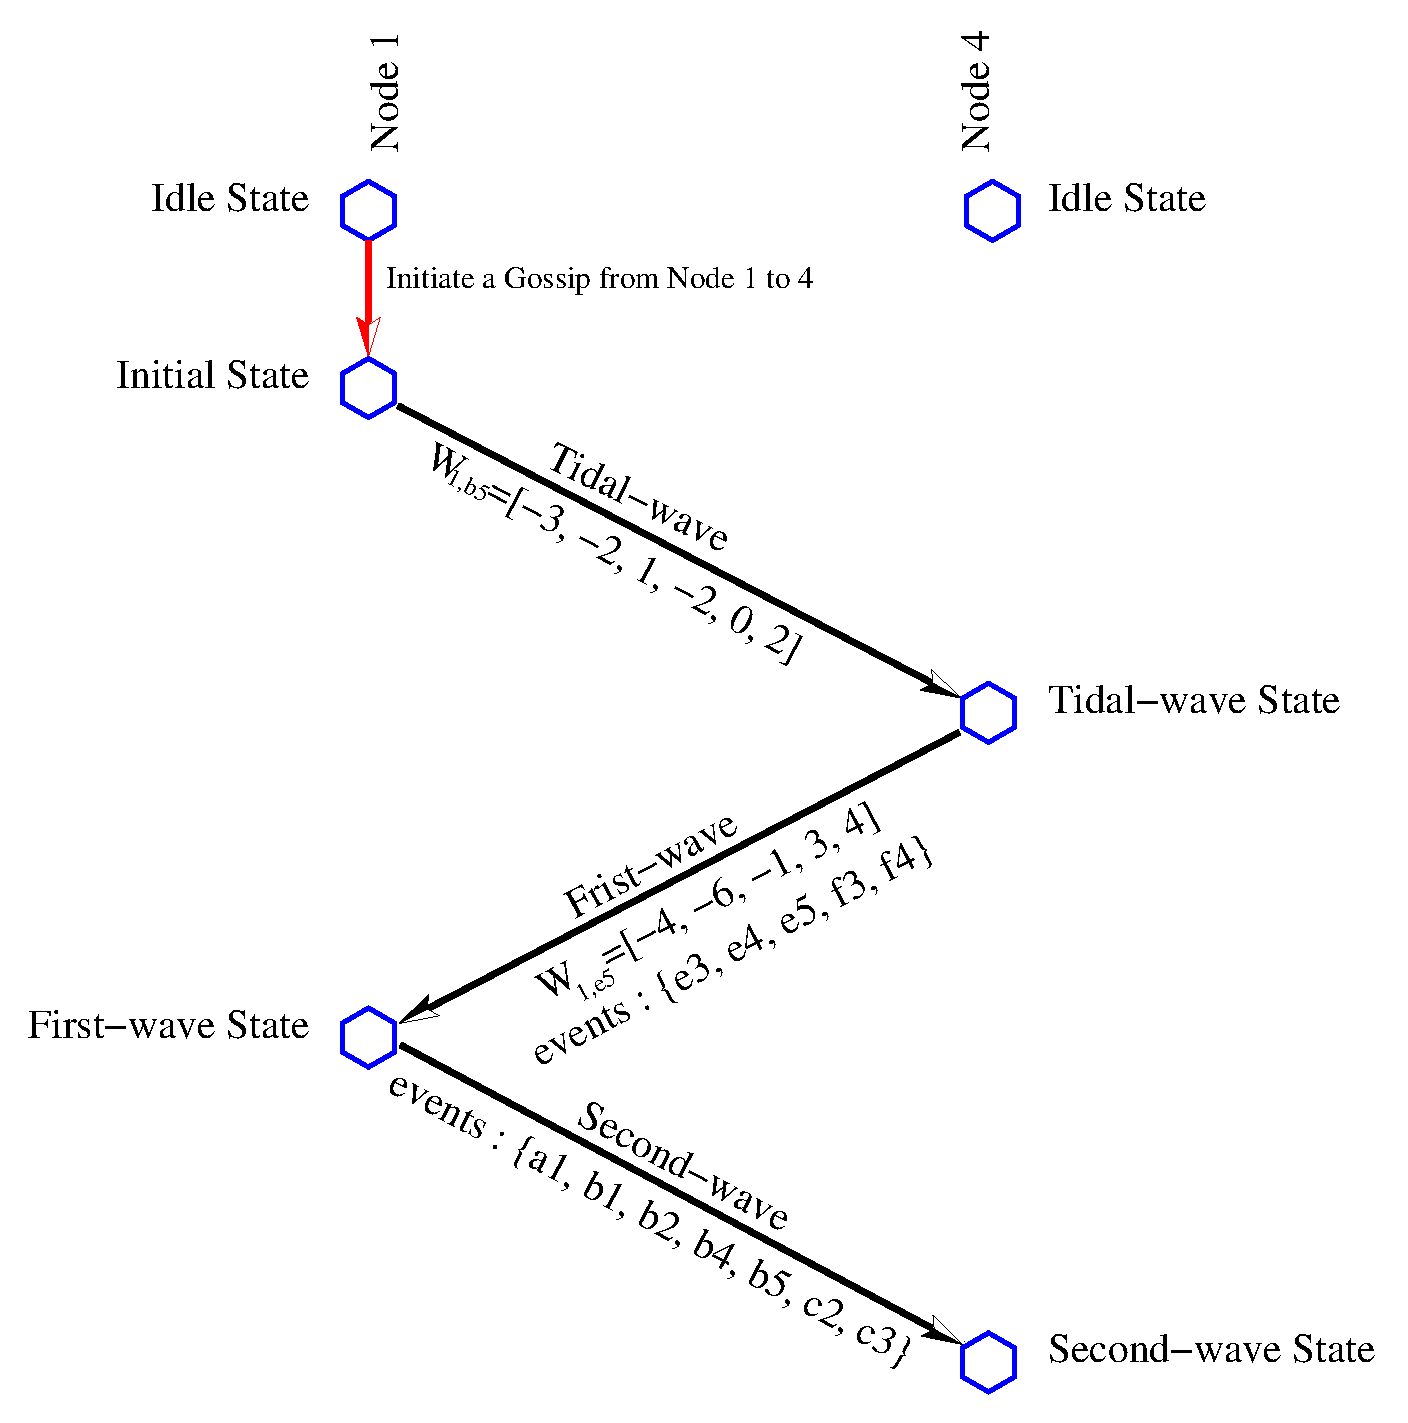
\includegraphics[width=0.7\textwidth]{fig/wavefront_communication.eps}
	% 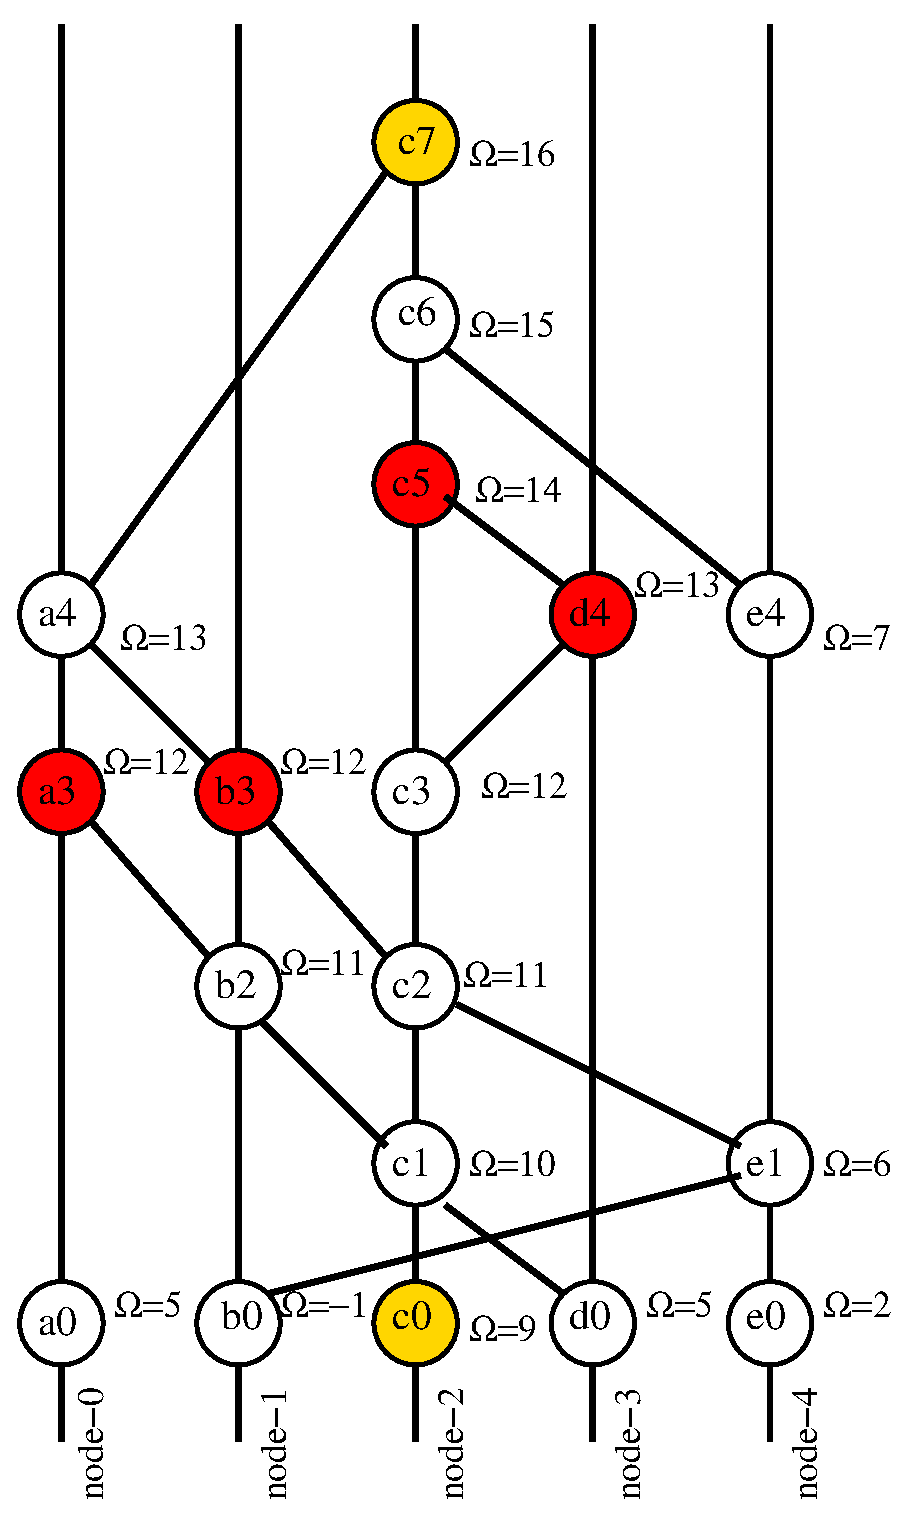
\includegraphics[width=0.45\textwidth]{fig/wavefront_and_order_small_no_alt.eps}
	% wavefront_and_order.eps: 3358x4625 px, 300dpi, 28.43x39.16 cm, bb=0 0 806 1110
	%\caption{Hashgraph with altitude(A) and parameter $\Omega$}
	\caption{Wavefront communication state}
	\label{fig:wavefront_communication}
\end{figure}

